\chapter{Networking the News}

In the previous chapters I outlined how archives, and critical readings of them, have expanded from fixed and graspable entities to a suite of interconnected parts, constantly shifting and adapting to new information. The web, when seen as an archive of archives, is itself ``an active and evolving repository of knowledge,'' rather than a fixed, bordered entity or set of categories.\autocite[2]{chakrabarti_mining_2003} This chapter hones in specifically on the structure of news stories and publishing archives, and the ways online publishers and legacy news outlets are treating their digital and digitized archives in this new era of continuous reclassification.

% “The searchable archive and classified ads can help each newspaper become a information databank in addition to its role as a deliverer of news. The hyperlinks have changed the newspaper from a single source of information into a hub of information networks without a clear ending point.” -- "Trends in Online Newspapers"

In the publishing world, recent years have seen two simultaneous trends that point to a fundamental shift in the function of mainstream news on the web, and a corresponding reformulation of the roles and practices of journalists. First, some new digital publishers are championing an ``explainer'' model of journalism. While explaining the news is nothing new (there has been a Pulitzer for explanatory journalism since 1985), explainer outfits take it a step further; featuring headlines like ``Everything you need to know about the government shutdown'' or ``40 charts that explain money in politics,'' explainer journalism aims to be ``as good at explaining the world as it is at reporting on it.''\autocite{klein_vox_2014} Second, legacy publishers have led a new focus on renewing and reanimating their historical archives. Whether they're cherry-picking and republishing old curiosities, providing subscribers with an interface to dive in and leaf through, or leading automated and crowdsourced projects aimed at organizing and structuring old content, legacy media has jumped at the chance to offer something that their born-digital rivals can't: a new take on providing context, a source for research and remix, and a trove of institutional memory and brand history.

These two trends reflect a new online media landscape, one which has seen journalists adapt by amplifying their role as explainer, verifier, and context provider rather than news breaker or scooper. The newsrooms that employ these journalists must adapt in turn. Publishers have a newfound opportunity to thrive in the information industry, but in order to compete in an information ecosystem currently dominated by Silicon Valley and Wikipedia, this new mentality cannot be simply verbal or piecemeal. It requires updated technologies \emph{as well as} cultural change.

Journalism has always hung in the balance between providing the facts and weaving a narrative. Michael Schudson frames the rise of popular newspapers in the 1890s as a pull between two journalisms, one telling ``stories'' and the other providing ``information.'' A fast-paced breaking event requires quick information, while contextualized longer-form histories and multimedia are more likely to serve an ``aesthetic'' function.\autocite[89]{schudson_discovering_1978} Journalists sometimes draw a similar divide between ``stock'' and ``flow'': the constant stream of information built for \emph{right now}, versus the durable, evergreen stuff, built to stand the test of time.\autocite{sloan_stock_2010} These are distinct but overlapping functions, and publishers often conflate the two. After all, longform stories also contain a great deal of information, even if that information is presented in a wall of text. In the digital age, the divide between stories and information can be blurred even further if we start to consider a news story as a curated, contextualized, and linked collection of facts and information. Through this framework, we might see structured and archive-oriented journalism begin to emerge as a hybrid of technology adoption and journalistic practice.

As such, this chapter is divided into two sections, one cultural and the other technical. First I will outline the origins of archive-oriented and explainer journalism, suggesting that the rapid proliferation of new content and connections have fundamentally altered journalism's roles and practices. The second section will consider the ways that publishers can adopt a technical infrastructure to support these new roles, first by analyzing in detail the architecture of a digital news story, then offering frameworks, tools, and techniques that might help to link archives and structure stories for future archival value.

\section{Context in context}

In newsrooms, the archive is traditionally known as ``the morgue'': a place where stories go to die. But new technologies and conditions have led to many recent attempts to reanimate the news archive, and there seems to be an ``archive fever'' developing amongst news publishers. Nicole Levy wondered if 2014 is ``the year of the legacy media archive'' in a story about \emph{Time} magazine's archival ``Vault.''\autocite{levy_time.com_2014} She points to \emph{The Nation}'s ``back issues,'' \emph{The New Yorker}'s open archive collections, and the \emph{New York Times'} TimesMachine as examples of old publishers endeavoring to use their rich histories to create something new. Back archives like \emph{Harper's} and \emph{National Geographic} are held up as examples of combining rich content with historical context, improving credibility and brand recognition in the process.

The \emph{Times} closely examined its own archives in its celebrated, leaked \emph{Innovation} report of 2014, suggesting that a clever use of archives would enable the Gray Lady to be ``both a daily newsletter and a library.''\autocite[28]{_innovation_2014} The report suggests that arts and culture content, more likely to be evergreen, could be organized by relevance instead of chronology, and that topic homepages should be more like guides than wires. It also enumerates successful experiments with repackaging old content in collections, organized by categories and themes; users could also create collections of archival stories, allowing reader interactivity without risk to the \emph{Times} brand. The report argues that by creating ``no new articles, only new packaging,'' the \emph{Times} could easily give new life to old content.\autocite[34]{_innovation_2014}

Along with the archival trend, we have recently witnessed an uptick in explainer journalism and an intense focus on providing context for online readers. Explainer journalism aims to take a step back from the immediate news event and place it in a larger phenomenon. It reflects a deep shift in the roles and practices of online journalists: as news is increasingly broken and scooped on blogs and social media, journalists are increasingly becoming summarizers, filterers, and context providers. In the archive and explainer movements, we see a pattern among some news outlets attempting to evade and reconsider the news cycle's obsession with speed and feeds, focusing instead on building structures and sustainability into journalism---in other words, on nurturing the archive in order to produce deep, contextualized stories. As many publishers emphasize the potential value of archives and context for the future of digital journalism, this moment is rich for closely examining this connection. By comparing the challenges of legacy media archives and newer forms of explainer journalism, we can gain a sense not only of how print and digital media differ as objects and media texts, but also of how journalistic practice has changed across both sectors.

Journalism has, of course, changed drastically since it moved onto the web. When a newsworthy event occurs now, it is likely to appear on social media within seconds, broken by eyewitnesses with cell phones rather than a reporter with a mic and camera crew. Alfred Hermida calls this phenomenon ``ambient journalism'': news now happens continuously, and it comes from everyone.\autocite{hermida_twittering_2010} This is especially true for distant events that are hard for newsrooms to cover in person; as foreign bureaus close around the world, this is an increasingly normal reality. Some citizen journalism initiatives are attempting to codify and normalize this new form of news production;\autocite[See][]{zuckerman_international_2010} but wherever it's published, this leaves mainstream journalists out of the breaking news loop. Reporters are relegated to picking up the digital pieces of stories as they are happening. Finding themselves in front of a computer for both reporting \emph{and} writing, a journalist's job now depends on strong online research skills as much as following beats and interviewing sources.

Mark Coddington sees journalists as moving away from ``what they consider the core of `reporting,'\thinspace'' while non-professionals are moving towards it.\autocite[682]{coddington_defending_2014} Gathering and breaking the news is a losing battle for mainstream journalists, and increasingly journalists are justifying their profession in different ways. Reviewing reporters' language around the WikiLeaks document trove, Coddington argues that journalists ``cast themselves fundamentally as sense-makers rather than information-gatherers during an era in which information gathering has been widely networked.''\autocite[678]{coddington_defending_2014} In discussing their value in the WikiLeaks case, journalists emphasized ``providing context, news judgment, and expertise.''\autocite[689]{coddington_defending_2014} Others noted similar trends and tendencies, even many years earlier; Kovach and Rosenstiel's \emph{The Elements of Journalism} quotes Xerox PARC director John Seeley Brown's assertion that ``what we need in the new economy and the new communications culture is sense making.''\autocite[19]{kovach_elements_2001} Journalist Amy Gahran agrees: ``today's journalists can---and probably should---consciously shift away from jobs that revolve around content creation (producing packaged `stories') and toward providing layers of journalistic insight and context on top of content created by others.''\autocite{gahran_swimming_2008}

Rather than being completely new, this trend is a sort of warped resurgence of traditional journalistic practices. Dan Gillmor praises legendary journalist I.F. Stone for his ``old-fashioned reporting,'' which Victor Navasky describes: ``To scour and devour public documents, bury himself in The Congressional Record, study obscure Congressional committee hearings, debates and and reports, all the time prospecting for news nuggets (which would appear as boxed paragraphs in his paper)\ldots He lived in the public domain.''\autocite[3-4]{gillmor_we_2006} These are librarians' verbs---scour, devour, bury, study, prospect---and the techniques don't seem so old-fashioned now. Schudson noted a turn towards interviewing as the primary journalistic technique in the late 20\textsuperscript{th} century, but new affordances in computer-assisted reporting---such as social media analysis tools and document repositories like DocumentCloud---have brought a resurgence of document-oriented sourcing. The ``holy trinity'' of newsgathering objects that media professor C.W. Anderson identifies---observation, documents, and interviews---has recently tipped back towards documents.\autocite[680]{coddington_defending_2014}

But in addition to repackaging original documents, many journalists are now repackaging other journalism. In a 2013 study, Anderson compares the practices of ``serious journalists'' and the news aggregators who republish them, to look for the boundary line in professionalism between original and repurposed content. Journalism and aggregation are generally taken to be at odds when considering newsroom expertise, but Anderson finds specific and often journalistic skills needed to be an aggregator. Calling them ``hierarchizers, interlinkers, bundlers, rewriters, and illustrators of web content,'' he suggests that \emph{news judgment} is their fundamental skill.\autocite{anderson_what_2013} News judgment is one of the core journalistic skills that Coddington identifies, and it undoubtedly requires an editorial eye. Meanwhile, ``serious journalists'' increasingly explain and contextualize breaking and ongoing news in an aggregational fashion. Joel Achenbach of the \emph{Washington Post} wrote in 2014 that ``Journalism is aggregation''; he noticed that in conducting rushed interviews with expert sources, he was doing the same skimming, lifting, and summarizing of his sources that aggregators do with theirs.\autocite{achenbach_journalism_2014} In a Reddit conversation with New York Times media columnist David Carr, a reader asked if Carr was ever frustrated by news aggregator Gawker stealing traffic from his original writing; the \emph{Innovation} report likewise laments a 161-year-old archival \emph{Times} story that went viral on Gawker rather than the \emph{Times}.\autocite[28]{_innovation_2014} But Carr replied by pointing out that Gawker was starting to create original reporting, while the Times itself is dipping into types of aggregating.\autocite{carr_iama_????} These professional lines seem to be increasingly blurred.

From the perspective of a digital media archaeologist, a web historian, or a software engineer building search algorithms, the difference between journalism and aggregation is that aggregating leaves a trace. It does so usually in the form of a hyperlink (if the aggregator is being friendly), or a tag, quote, or snippet from the original article. This trace is crucial; it not only helps search engines understand influence, but it forms a dialogue and joins a network, allowing it to be resurfaced and mined in the future. This could be one reason that aggregators often win out over original sources in battles over traffic. This is not to say that aggregating is better or more influential than original reporting---only that it plays by the citation rules of the web, and is rewarded for it. Of course, sometimes journalists can't publish or link to their sources, and it would be unduly cumbersome for a reporter to publish hours of audio transcripts just to provide context, not to mention the complications of anonymous or off-the-record comments. Some bloggers and new journalists suggest that it is a best practice to publish every source in full context, but forcing a journalist to obsessively link to every source risks stifling journalistic practice. All the same, the hyperlink and the tag combine to allow for a new standard of citation, reference, and context provision for news on the web, and journalists would be well served to think about the explicit and latent links buried within their stories.

While I will consider the more technical aspects of links and tags in section 4.2, this sets the stage for considering how the dual trend of archiving and explaining reflects a new focus in the work of digital journalists. While many have discussed the blending of journalist and computer scientist in so-called ``data journalism'' (for instance, consider the dual journalism and computer science degree now offered by Columbia University), I also posit a link between journalists and librarians/archivists in the current moment's focus on context and explanation. Emphasizing such a connection could lead to a journalistic focus on both more rigorous research and citation skills, and long-term information sustainability.

\subsection{The archive drive}

Legacy media's turn to archives is a reflection of many uncertainties about the future of journalism. After all, it seems antithetical for news to focus on history; news has forever been focused on the \emph{new} and \emph{now}. The pace of \emph{now} has only accelerated online, as newsrooms shift from daily or weekly print schedules to continuous publishing and posting cycles. For a reporter, this creates a work environment of real-time frenzy; a reporter might have live statistics on her article's performance in one window, while she furiously scans a flurry of tweets looking for her next scoop in another. It's no wonder that newsrooms haven't traditionally focused on their archives; for today's reporter, media loses value with each passing second.

But this everyday practice---manifested in real-time feeds, streams, and notifications on Twitter, Reddit, and RSS---is at odds with the plethora of old stories, images, facts, and quotes that are perpetually accessible on a publisher's website. Some stories are part of larger story arcs that have lasted for years, while others lie dormant for decades before resurfacing due to new facts or a notable anniversary. These old stories are continuously updating too; if you click on one or add a comment, you register another pageview or annotation in the database. The past and present collide in the digital news database. Archived stories are consistently changing, acquiring new clicks, new links, new topics and tags to reflect ongoing events. Drawing on my discussions of containment and connection in section 2.2, this strikes a sort of paradox, where the archive contains the object but keeps forging connections. This paradox emphasizes the continual relevance of the archive to the present, and the need to balance the steady stream of news with a dose of history.

The web's archival affordances are crucial for media scholar Peter Dahlgren, who sees archivality as one of the five components of the ``media logic'' of cyberspace.\footnote{Mark Deuze only names three ``logics''---hypertextuality, multimediality, and interactivity---but Dahlgren adds ``figurational'' and ``archival.''} For Dahlgren, archivality forms a symbiosis with hypertextuality---another web logic---which enables new and more usable archives. The end result is that ``users of cyberspace for journalism are in principle no longer so bound to the present.''\autocite[66]{dahlgren_media_1996} Even as reporters are focused on \emph{right now}, their users might be more interested in \emph{back then}. But this is not necessarily borne out in publishers' insights about their readers. Most publishers are sure that archives are valuable, but they have vague answers for exactly \emph{why}. Moreover, the answer could be different for each publisher. While the \emph{Times} asserts a competitive advantage over born-digital upstarts like Vox and BuzzFeed, most do not go beyond suggesting that it is a unique and more or less rights-free repository of content. The University of Missouri's Reynolds Journalism Institute offers that ``It is difficult to calculate the full value of news archives given the countless hours of reporting and editing they distill, not to mention the treasure they represent in terms of their community's cultural heritage.''\autocite{mccain_saving_2014} They also suggest that archives ``serve as a form of institutional knowledge,'' allowing new journalists to get up to speed on the historical context of an ongoing story. This is especially crucial for new hires at highly local or specialized publications, whose archives often contain a unique and unmatched amount of information on a certain community or genre.

% Retro Report? http://www.niemanlab.org/2014/05/the-third-draft-of-history-retro-report-looks-back-at-media-hyped-stories-of-the-recent-past/

% JSTOR? http://www.niemanlab.org/2014/10/opening-up-the-archives-jstor-wants-to-tie-a-library-to-the-news/
% The digital academic library JSTOR is hoping to introduce historical, academic, and scholarly insights to ongoing news items through its new site \emph{JSTOR Daily}; here again, we see the increasing media collision between news and history. ``JSTOR Daily won’t be breaking any stories, Halley said, explaining that she hopes the site will “provide the backstory to the news.''

The Reynolds Institute led a 2014 survey of 476 news websites, finding that 88--93 percent of them highly value their archives. But the origins of this study are telling; the school's \emph{Columbia Missourian} paper lost 15 years of stories and seven years of images in a single 2002 server crash. According to the study, despite the nearly universal lip service paid to archives, about a quarter of news websites had lost significant portions of their archives due to technical failure. Missouri journalism professor Tom Warhover provides a series of examples to emphasize the devastation: ``You can't offer up a comprehensive product to sell---your archives---if they aren't complete. You can't be sure you've really vetted a candidate for school board or city council. You can't find those historical pieces from events that now are historic and worth reporting again on anniversaries.''\autocite{mccain_saving_2014} These examples showcase the latent and often hidden value of the archive, not only as a product but as a deep journalistic resource and form of institutional memory.

The \emph{Times} asserts that ``our rich archive offers one of our clearest advantages over new competitors,'' though they have done little to mine its value, ``largely because we are so focused on news and new features.''\autocite[28]{_innovation_2014}  The \emph{New Yorker} also found some success in summer 2014 by opening up its archives while it experimented with a new paywall. As readers raced to download classics written by Ariel Levy, Philip Gourevitch, and Kelefa Sanneh, the announcement got the public talking about the forthcoming redesign and the rich history of the \emph{New Yorker} brand. While the archive summer saw decent engagement, the work has paid off since reinstating the paywall; web editor Nicholas Thompson says that in the summer ``there wasn't a massive increase\ldots[w]hat's weird is we launched the paywall, and \emph{then} there was a massive increase.''\autocite{ellis_after_2015} While the \emph{New Yorker}'s success is on the back of its redesign and paywall, its archive played a foundational and unmeasurable role.

Now the \emph{New Yorker}'s archives are back under lock and key, as they are for most publishers. Newspapers see a synergy between digital archives and paywalls, considering that the archives could be a valuable draw for subscribers, and especially an enticement for researchers who might be willing to pay for a subscription. The typical archive diver is seen as a dedicated browser or dedicated searcher; interest in the archive is already assumed at the outset. For the rest of the population, the archive is locked away. This runs counter to the linking and sharing economy of the web; as many publishers have experimented with the tension between linking and locking, the archives have remained firmly locked away. Joshua Rothman, the \emph{New Yorker}'s archives editor, thinks that the most crucial element of enlivening the archive is to simply make it available in the first place; it is hard to predict or control when an old story will return to relevancy or gain new attention, but it cannot happen without users being able to find and access it.\autocite{rothman_interview_2015} This suggests a need to treat archival stories with a nuanced paywall approach.\footnote{Legacy publishers are also often stifled by long-term contracts with archive services like ProQuest; some of these limitations are not for a lack of creativity, but rather legality.} Most publishing archive landing pages hardly even allow even a ``preview'' of the archival content or interface, and the more nuanced paywalls (for instance, ones that let readers access six stories a month) are virtually nonexistent for archives. Some publishers, \emph{Time} included, will lift the paywall on certain ``whitelisted'' stories, ones that might have jumped back into relevance and that new stories are linking to. This is a start, but defaulting to locking away limits the possibilities for serendipitous encounters with archives. Sometimes publishers have long-term agreements with professional archive services like ProQuest, which likewise stifle creativity.

Still, archives don't directly drive clicks, and legacy publishers have well-documented financial troubles, so their archives have taken a hit. While most newsrooms have a library or research center, the ranks of newsroom librarians are dwindling. Over 250 news librarians lost their jobs in the U.S. from 2007 to 2010, and membership in the Special Libraries Association News Division has steadily dropped. Some news libraries and research centers have been completely shut down, outsourced to vendors like LexisNexis.\autocite{silverman_endangered_2010} As newspapers endeavor to enter the information age, it is a shame to see them losing their information professionals. Librarians provide crucial research and fact-checking skills. Amy Disch, chair of the Special Libraries Association News Division, speaks to the traditional division of skills between reporter and librarian in the newsroom: ``We can find the information in a lot less time because we know how to drill down in a database. We know good sources to go to where you can quickly find information, so we can cut a lot of time for [reporters] and leave them to do what they do best, which is interviewing and writing. I have my specialty, and they have theirs.''\autocite{silverman_endangered_2010} Librarians are also the shepherds of the archive, tagging and structuring new stories and continuously maintaining them as history develops. Most major news organizations no longer have the library manpower to manually review every new story for proper tagging and indexing; this also points to their limited capacity for maintaining the topic taxonomy, or experimenting with new indexing and metadata projects.

% Nora Paul concludes with a call to reuse content via hyperlinking: ``It used to be called the morgue, then the library, now, in lots of places it's the news research center. But what the electronic products newsroom needs is an information recycling plant.''\autocite{paul_1995}  ``Rethink reporting as a layering of news.''
% Similar to Joshua Rothman's quote about the archive existing to avoid repeating work

A few publishers have thrown up their hands altogether, relying on third-party services to organize and provide access to their own archives.\autocite{romenesko_u.s._2014} Reporters might suddenly see old stories disappeared from the web, locked away behind services like ProQuest and LexisNexis. Such services provide fast and effective text search at low cost; but at what cost to an organization's brand, legal rights, and sense of history? A story is not just text, and increasingly, an archive includes images, videos, charts, maps, interactives, facts, statistics, quotations, comments, and annotations. This will become increasingly important as media evolves in a ``post-text'' web; the next generation of media companies cannot rely alone on text search to access their past.\autocite{salmon_why_2014}

Due to the ambiguous value of news archives, it seems to go without saying that old stories should be saved, but it's harder to know exactly what to do with them. Saving them turns out to be the expensive part; the cost of digitizing, indexing, and hosting gigabytes of old content is no small investment. Some publishers stop here: they might offer a search interface for staff members and researchers, as well as a PDF-style flipbook view that allows obsessively curious subscribers to leaf through the ``original'' paper or magazine. These interfaces will serve those with a research interest or innate curiosity, but this only scratches the surface of the archive's potential as a serendipitous window into past insights for journalists and casual readers alike.

A publisher's archive will often turn up in specific articles geared towards history. At \emph{Time}, archive editor and curator Lily Rothman (no relation to Joshua Rothman at the \emph{New Yorker}) digs out stories and quotes from the history of \emph{Time}, ranging from historical interests (``Read TIME's Original Review of \emph{The Catcher in the Rye}'') to ephemeral oddities (``13 Weirdly Morbid Vintage News Stories''). Editor Samuel Jacobs likened Rothman to a radio D.J., highlighting singles from the archive to entice readers to pay for the whole collection.\autocite{levy_time.com_2014} Other historic deep-dives might occur in weekly columns or ``long history'' forays by individual journalists. A Sunday Times article, for instance, might take a historic look at a particular person, neighborhood, or community. These projects have a chance to draw attention to the past through curation as well, by drawing out and resurfacing old stories, photographs and statistics; such projects are a promising start, but they tend to be isolated endeavors, relegated to a single story. Sometimes willfully nostalgic, they do not bring the archive fully into dialogue with ongoing events, whether in the research or design process.

% Maybe more debate here about different ways publishers currently use archives: "curios" that relate to today's news, random dives like "isn't it funny they had cat pictures in the 1920s too?", or just showcasing the best writing a la New Yorker
% Other examples? Local interest stories etc. e.g. history of Whitey Bulgur, Boston's bids for the Olympics, or neighborhood deep-dives.

Topic pages suffer from lack of organization and explanation as a result. Imagine navigating to a topic page, such as one of \emph{The New York Times'} over 5000 pages ranging from ``A.C. Milan'' to ``Zimbabwe,'' and seeing a map or timeline of the most important stories in the \emph{Times'} history. What about viewing a network of stories as a graph of influence and dialogue, or pulling out the most relevant quotes, images, videos, or facts from the story to highlight for the user? If the \emph{Times} hasn't written about A.C. Milan in a while, they could suggest a story about a rival soccer team, or Italian football clubs in general. Search interfaces and topic pages can function like research librarians, retrieving information and context, instead of a list of stories and items. Like any good librarians, if the information is not at hand, they could point the reader towards where to find it.

Such a future requires smart use of indexing and metadata schemes, which I will consider in the following section; but it also requires a cultural shift in both the conception of the archive's audience and the ways that journalists think of their stories' value. For now, legacy publishers seem to know well that their archives are a competitive advantage, and an asset that sets them apart from born-digital upstarts. \emph{The Nation}'s editor and publisher Katrina vanden Heuvel suggests that ``a clever use of archives is kind of an explainer 2.0,'' directly placing the two movements in comparison and competition.\autocite{levy_time.com_2014} But ironically, publishers with brief histories are the ones that have been emphasizing historical context. It's possible that in aiming to revitalize the archive and blend the present with the past, archive-oriented publishers might be bringing past conventions back into the present.

\subsection{Explaining the news}

The \emph{Times'} \emph{Innovation} report names Vox as one of its direct competitors and threats, a new digital upstart innovating with new models of news production. This was an auspicious start; at the time of the report, Vox had not even launched. Its parent company, Vox Media, already counted several special interest sites in its ranks, but Vox was its first general interest property. Vox also had a few big names behind it already, namely co-founder Ezra Klein, who left his position at the helm of the \emph{Washington Post}'s Wonkblog to start this digital outlet. Vox has quickly become a fixture of digital start-up news, as well as the poster child of the explainer movement, along with Nate Silver's \emph{FiveThirtyEight} and the \emph{Times'} own Upshot venture. By taking a broad, data-oriented stance on reporting, Vox aims to infuse deep context and data into its journalism, technology, and business decisions alike. Vox's signature feature is its ``card stacks'': collections of reusable and editable snippets of facts, quotes, maps, and other media, collected and synthesized by a journalist. With titles like ``Everything you need to know about marijuana legalization'' or ``9 facts about the Eurozone crisis,'' the stacks subdivide into question- and statement-driven ``cards,'' like ``What is marijuana decriminalization?'' or ``Debt didn't cause the crisis.'' Readers can navigate sequentially, or leap from card to card. The final option on each card is the same: the ``Explore'' button takes the reader back to the top of the stacks.

The purpose of the card stacks is similar to many legacy institutions' reasons for protecting their archive: to avoid repeating work. For Klein, ``the biggest source of waste is everything the journalist has written before today.''\autocite{kaufman_vox_2014} Through the card stacks, we see a steady accumulation of a new kind of publishing archive, one oriented around questions and statements rather than topics and tags. The card stacks are not only a public-facing form of archive, they are a core feature of the Vox product; Vox is not just selling stories (content), but a story \emph{structure} (a container). This leads to a shift in the role of the journalists, who explain and contextualize as journalists always have, but with an eye towards updating the stacks as well as pushing new stories.

Klein has Wikipedia in his sights, suggesting in a \emph{New Yorker} interview that ``I think it's weird that the news cedes so much ground to Wikipedia. That isn't true in other informational sectors.''\autocite{coscarelli_ezra_2014} Wikipedia is the looming giant in context provision; publishers understandably ask how they could do any better without unlimited staff and budget. But Wikipedia is a generalist's resource, and its readings on more specialized and newsworthy topics can be dense and dry. Some topics, especially in science or medecine, assume a reader's technical knowledge from the outset. Linking to Wikipedia also, of course, takes the reader away from the publisher's site, at the risk of leading them down a rabbit hole of Wikipedia links in a quest for more context. Vox's card stacks are a sort of journalistic alternative to Wikipedia, a wiki ``written by one person with a little attitude,'' as co-founder Melissa Bell puts it.\autocite{kaufman_vox_2014} This allows for customized context, created ``in-house.''

Klein envisions a virtuous cycle of curiosity and information: ``the card stacks add value to the news coverage. And the news coverage creates curiosity that leads people to the card stacks.''\autocite{coscarelli_ezra_2014} The symbiosis between news coverage and cards is clear for journalists who need to quickly fact-check and contextualize, but the magical formula of news coverage that ``creates curiosity'' for a reader is a vague and difficult goal. Some think that newsreaders are just looking for news, not information and context. Others believe that Vox is diving too deep into the information space; given that even teams of trained librarians struggle to organize information, how can a team of journalists hope to keep up? They have ``a huge challenge, due to the rapid decay of facts,'' according to Craig Silverman, who suggests that Vox could use a librarian.\autocite{silverman_why_2014} In order to be feasible, each card needs to be both independent and linked; the cards are adoptable as standalone pieces, but they also have to add up to a coherent narrative for linear reading. How can a journalist keep a card independently updated, and know that it is up-to-date? Consider, for instance, Vox's card on marijuana legalization, which has already been updated 40 times between April 2014 and February 2015.\autocite{lopez_everything_????} Scientific research on marijuana's health effects is known to be limited; what happens to these preliminary studies when they are replaced by more rigorous ones? How will a journalist be alerted when a new research paper debunks an old fact or figure? What happens to such a card if marijuana becomes legalized across all 50 states?

But Vox doesn't say their cards contain everything, just ``everything you need to know.'' While the card stacks might be Vox's technological foundation, this economical, itemized, somewhat glib approach to contextualizing the news is its journalistic signature. Some critics have lambasted the site for the hubris of its mission; it doesn't get much bigger than ``explaining the news,'' and it might be best left to a distributed group of subject-matter experts (or the public, in Wikipedia's case) rather than a core of time-strapped journalists who are often distant from the topics that they cover. Vox has already gotten some things wrong, and Deadspin gleefully and sometimes unfairly picked apart a full 46 Vox corrections from its first year.\autocite{draper_46_2014} Others question the site's tone; music journalist David Holmes lamented that Vox's model gives the reader ``just enough information\ldots to \emph{sound} smart,'' appealing primarily to ``the type of person who's afraid of sounding gauche at your next dinner party.''\autocite{holmes_how_2015} ``Everything you need to know'' sounds final, running counter to the very idea that knowledge is interlinked, flexible, and intersubjective: everything \emph{who} needs to know? Vox's style of explainer journalism can feel cold and distant; it's more likely to explain why people are excited about a new movie than to get \emph{you} excited about the movie.

Vox is far from the first or only explainer, and the concept of explaining the news is a core journalistic principle. A 2001 Pew Center survey of newspaper editors concluded that they wanted to be ``news explainers'' first and foremost, ahead of ``news breakers'' or ``investigative watchdogs.''\autocite{pew_research_center_journalism_2001} But in a 2008 article called ``National Explainer,'' Jay Rosen accused editors of not staying true to their mission: journalists are not good at explaining the news and providing context.\autocite{rosen_national_2008} Instead, they focus too much on incremental and episodic updates, many of which go over the head of readers who haven't been following. Rosen likens the process to pushing software updates to a computer that doesn't have the software installed.

Journalists ``don't do a very good job of talking about the beginning and what got us to this point where it became news,'' according to Alex Blumburg.\autocite{rosen_national_2008} Even the occasional explainer that gets it right ends up in the flow of the same old information; Rosen argues that explainers like David Leonhardt's credit crisis piece in \emph{The New York Times} ``should have been a tool in the sidebar of every news story the Times did about the mortgage mess.'' The little ``what's this?'' link that pops up on occasional news websites is ``not about web design. That's a whole new category in journalism that I fear we do not understand at all.'' Rosen went on to create explainthis.org, a site for people to admit what they don't know; journalists, the site promises, are ``standing by.''\autocite{_explainthis.org_2010} Now defunct, explainthis.org was like a library reference desk, staffed by the public and monitored by journalists. A peer of StackOverflow and ancestor to Quora, it is organized around questions rather than topics, discussed by the public and monitored by journalists. It requires someone to be curious enough to ask the question, however. Rosen and Klein tout the explainer's role as a driver of deeper interest in a topic, but here we're already expected to be interested.

At a 2010 South by Southwest conference panel called ``Future of Context,'' Rosen outlined the reasons explanation is needed and why it wasn't taking off. He cited both design and institutional problems; the prestige and real-time excitement of breaking (rather than explaining) news, as well as the explainer format getting lost in the shuffle of other news items.\autocite{rosen_news_2010} Metrics like clicking, watching, and even spending time on a site are not measuring the level of understanding or knowledge gained. Panelists like NPR's Matt Thompson and Apture CEO Tristan Harris turned more towards the systems and technologies that compound the problem. Harris offered an ``object-oriented journalism'' model, which asks journalists to ``think like an engineer'' and never do work they can't reuse. Thompson considered the potentials of a context-oriented website; how could you take a topic page and make it more than a random collection of links? What would a site look like if it were structured around systems instead of stories?\autocites[See][]{rosen_news_2010}{myers_liveblogging_2010}{hu_contextualizing_2010}

Vox is not a complete shift into this territory, but it's a start. The card stacks might initiate a subtle shift in the ways that journalists think about the value of their content. A reporter who is writing about a new study on marijuana's health effects could do so by editing an existing card, or by writing a new card; this card could also be published to Vox as a standalone story. If the existing card already featured a few other helpful background facts, or a nice map or infographic, the reporter could attach it to the new story too. This not only saves time and adds value to the story, but it produces a subtle shift in the journalist's practice; the story is itself a collection, and it's part of other, bigger collections. The story is here to stay.

Vox has also experimented with another simpler but novel use of content: republishing evergreen stories. In December 2014, during a typically slow news cycle, Vox edited, updated, and republished 88 old stories from their archive.\autocite{yglesias_refreshing_2015} Some of these went through a heavy round of editing, while others were republished nearly as-is; in either case, no one seemed to notice that the content was old. Some stories that didn't draw readers the first time around experienced a second life. Executive editor Matthew Yglesias explains, ``On the modern web, content tends to arrive via miscellaneous streams rather than coherent chunks. So the meaning of strict chronology is breaking down regardless of what publishers do.''\autocite{yglesias_refreshing_2015} This approach is a sort of workaround of the traditional stream-based publishing format; since we haven't found a good way to differentiate evergreen stories in our feeds and streams, Vox is just pushing them repeatedly. But the experiment was enough of a success that writers continue to refresh old content, united in Vox's quest to become a ``persistent news resource.''\autocite{yglesias_refreshing_2015}

In this section I have aimed to outline the ways in which journalistic practice is changing on the web. Journalists are adopting the role of sense-maker, taking a step back from the immediate event and endeavoring to place it in a larger phenomenon. This is manifested in a corresponding reliance on documents more than interviews and observation, which blurs the line between journalist and aggregator and offers a new conception of a news story as a document-driven collection of linked information.

\section{The size and shape of stories}

Here I will turn to the technical challenges inherent in linking this information, first by examining existing practices in digitizing and researching in digital archives, then by looking to the ways that digital stories might be structured, treated, and archived as a result. 

As I outlined in previous chapters, every archive has its own size, shape, and properties that the digital has complicated and exploded. The same goes for stories, too. The structure of a story and conception of its shape has rapidly changed. Even a typical newswire that delivers last night's sports scores---seemingly an unchanged art from its paper-news origins---now offers new context, such as an interactive chart with the box scores, or inline links to the teams' pages. Journalists have sometimes been slow to adopt these hypertextual and interactive elements, but as some more recent studies show, the pace is on the rise.\autocites[See, e.g.,][]{coddington_building_2012}{coddington_normalizing_2014}{larsson_staying_2013}

Consider a typical old and archived newspaper story, such as the \emph{Times'} March 14, 1969 feature ``Lindsay Warned on School Budget,'' available on the TimesMachine. It appears on the paper's front page, sharing space with news of the safe return of the Apollo 9 mission, as well as eight other stories covering Washington, Russia, and local New York affairs. The story has several components: a title, a subtitle, a lead paragraph, and four distinct sections, spanning two pages. Its digitized version on TimesMachine exposes much of this structure: the title, subtitle, lede, byline, publish date, and page numbers all appear as separate fields in its metadata. TimesMachine also offers five ``subjects'' that the story belongs to: Education and Schools, Finances, New York City, State Aid, and Welfare Work.\autocite{bennett_lindsay_1969}

The TimesMachine is perhaps the most well-indexed publishing archive, but even these tags don't give a glimpse of the New York City public education system in the 1960s. Today's readers might be wondering who ``Lindsay'' is (the answer: New York City mayor John Lindsay, who served from 1966 to 1973), or the subtitle's ``Doar'' (John Doar, prominent civil rights lawyer turned New York Board of Education president). These missing background details leave readers in the dark unless they have been following the story all along, whether the reader is a New York-based newspaper browser in 1969 or a Canadian TimesMachine diver in 2015. The story is replete with facts and background information of its own, but it is all buried deep within the story.

Comparing it to a more recent local education story reveals interesting differences. In a story called ``New York Schools Chancellor Replaces 8 Superintendents,'' the \emph{Times} discusses the latest actions by Carmen Fari\~{n}a, the New York schools chancellor.\autocite{taylor_new_2014} The structure is different even in the first two words: Fari\~{n}a's name is hyperlinked, leading to a deeper piece from the archive on her background and management style. Other, more subtle shifts in language point to a focus on background and context as well; where the 1969 article simply referred to ``Lindsay'' or ``John Lindsay,'' its 2015 counterpart refers to ``former Mayor Michael R. Bloomberg'' even though he needs no introduction to most of today's \emph{Times} readers. A later reference to the ``Education Department'' links out to a Times Topic page about the New York City Education Department, allowing for curious or uninformed readers to see more articles and gain more background. These subtle shifts in writing style add new layers of structure and context to a news story, and allow it to be understandable both to less-informed readers and those who return to the story months or years later.

Also telling in these stories are the many original facts and figures: the names and districts of the eight superintendents being replaced, the names, titles, and relationships of major players in New York's education administration, and precise figures about the city's education budget and class sizes in 1969. But rather than entering this information into a database, reporters reveal them in their writing. Much of this information is then lost to future researchers and subsequent journalists. The challenge is to properly \emph{structure} this information so that journalists' research can stay fresh and updated, but without requiring onerous data entry or duplicate work.

We can look to computer and information sciences for useful tools, techniques, and approaches for mining this latent structured information. For instance, historical figures like John Lindsay and John Doar are what a computer scientist calls Named Entities; most news stories mention a series of interactions and relationships between newsworthy people, places, organizations, dates, and times, and each of these can be a named entity. For instance, a phrase like ``Barack Obama will speak to Congress on Wednesday,'' has two named entities---Barack Obama, and Congress---that can begin to give computers clues as to what a story is about, and what other stories are related to it. A story referring to his meetings with the Pentagon (another entity) is likely to be about federal defense and security, while another meeting with the Council on Environmental Quality is likely about clean energy. More subtly, a phrase like ``Barack Obama will speak to Congress on Wednesday, July 15'' adds another named entity: a date. This gives the phrase slightly more structure, which leads to more potential; an automated system could remind a reader on July 15 that Obama is speaking, or it could mine many stories' text for every time Obama has spoken to Congress, displaying it on a calendar or timeline. These small pieces of structure add up on a larger scale, offering many new uses for old news.

% Also: data journalism is not a new phenomenon, and old stories contain tables, facts, and figures to be mined for insight http://www.propublica.org/nerds/item/antebellum-data-journalism-busted-abe-lincoln -- good example both of old data journalism, and use of archives for new stories

In this section, I will first trace the stages and techniques for exposing and gathering insight from archives of news. This will start to reveal how actors and facts interact in a news story, and the size and shape that modern stories can adopt as a result. Then I will consider the potentials for new forms of organization by taking advantage of the structures and systems buried within news stories.

\subsection{The hypertext newspaper}

% Somewhere mention challenges of PDF-to-HTML
% Blustein 1999 “Hypertext Versions of Journal Articles”

Newspaper and magazine publishers prove an ideal study for examining the potentials of hypertext archives. Along with the subtle structure of stories, newspapers contain their own structures as well. Few readers go through a newspaper sequentially, paying equal attention to every article; instead the reader jumps around from page to page, skimming some sections for its raw information while reading longer pieces more deeply. A website homepage reads like a newspaper's front page, with snippets and teasers organized by general relevance that aim to draw the reader deeper. A given page can hold several articles organized by specific topics and subtopics, and an interested reader might be distracted or intrigued by a ``related article'' next to the one he came to read. Some works are categorized into sections---arts, sports, letters to the editor---while others might be paired with a certain advertisement or reaction article. These examples point to the inherently interlinked, ``jumpable'' nature of newspapers, and the endless potential for insightful metadata; newspapers might seem to naturally lend themselves to the digital world.

The typical newspaper's current architecture started as a response to a sort of historical information overload; the newspaper frontpage and summary lead paragraph, both solidified in 1870, were part of a broader trend towards ``helping readers to economize their scarce time in scanning a paper.''\autocite[254]{starr_creation_2004} Larger type, illustrations, and bolder headlines drew criticism for trying to grab attention, but they also directed and focused attention to the major stories of the day, allowing for nonlinear readings of a newspaper as a fragmented collection of stories, headlines, or ledes. A newspaper's layout and seriality therefore scaffold a pseudo-hypertextual structure, one that can be computationally mined for insights.\footnote{Some libraries and cultural heritage institutions are leading these endeavors, such as the Library of Congress' National Digital Newspaper Program, Europeana, and Trove.}

Given the print newspaper's proto-hypertextual status, it presents a unique metadata challenge for archivists. What metadata is worth saving and breaking down: the text, the subtext, the pictures? The photo or pullquote on the side? For some researchers, placement will be important (was an article's headline on the first page? Above or below the fold? Was there an photo, an ad, or a counterpoint article next to it?). Others could be focus on the newspaper itself over time, rather than the contents within (for instance, did a paper's writing style or ad placement change over the course of a decade?) Still others may be hoping to dive into coverage of a particular event across various journals. In each case, we can glean information from where and when it was published on the page. A newspaper is a very complex design object with specific archival affordances; their structure and seriality make them ripe for unique forms of automated analysis.

Old newspapers are rich archival documents for historians and scholars, because they store both ephemera and history. Newspapers also hold advertisements, classifieds, stock quotes, and weather diagrams. Many researchers rely on such ephemera---James Mussell calls it ``a key instrument of cultural memory''---so from the traditional archivist's perspective, everything needs to be considered ``stock,'' stored forever.\autocite{mussell_passing_2012} Paul Gooding, a researcher at University College London, sees digitized newspapers as ripe for analysis due to their irregular size and their seriality.\autocite{gooding_exploring_2014} In order to learn more about how people use digitized newspaper archives, Gooding analyzed user web logs from Welsh Newspapers Online, a newspaper portal maintained by the National Library of Wales. He found that most researchers were not closely reading the newspapers page by page, but instead searching and browsing at a high level before diving into particular pages. He sees this behavior as an accelerated version of the way people browse through physical archives---when faced with boxes of archived newspapers, most researchers do not flip through pages, but instead skip through reams of them before delving in. So while digital newspapers do not replace the physical archive, they do mostly mimic the physical experience of diving into an archive.

Still, something is lost when the physical copy becomes digital; the grain of history---the old rip, annotation, or coffee stain---is reduced to information.  As many theorists and historians remind us, too, a paper's physical appearance and content are closely linked together, so simply ``digitizing'' and newspaper changes it massively, reshaping a great deal of context.\autocites[See, e.g.,][388-389]{manoff_archive_2010}{mussell_elemental_2014} Richard Abel, a scholar of early U.S. and French cinema, breaks down the promises and challenges in generating archival ``big data'' in his research. Using archival resources like NewspaperArchive.com and GenealogyBank.com to access 1910s newspapers, he found ``a wealth of unexpected documents,'' but he notes the unreliability of completeness and searchability, the collapse of community, and the ``\emph{having been there.}''\autocite[6]{abel_pleasures_2013}

Old newspapers are also replete with images and advertisements, which offer a more vivid sense of history. Leafing through old pages of the \emph{Times} or \emph{Time}, it is the images and ads that jump out beyond the stilted text of news items. But tellingly, many news digitization projects, begun decades ago, focused exclusively on salvaging the text. This ignores substantial information in the archive, of course, and speaks to the shortsightedness of many projects aimed at digitizing the past. Images, advertisements, maps, formatting, and related metadata were all lost, and many of them are being re-scanned by publishers, at great expense, in order to properly atomize the archive and capture the details that they ignored years ago. This doesn't account for historical problems with tagging images; University of Missouri photojournalism professor Keith Greenwood found that many newspapers diligently archived their photographs for daily newspaper use, but did not tag items with public historical value in mind, rendering many of them useless as historical records.\autocite{greenwood_digital_2011} In a 2014 special issue of \emph{Media History} focusing on digital newspaper archive research, Nicole Maurantonio criticizes newspaper indexes for ignoring the visual in favor of text, ``propelling scholars down a misguided path.''\autocite[90]{maurantonio_archiving_2014}

Historical images are one of the greatest potential sources of engagement and revenue for news archives, and outlets like the New York Daily News, National Geographic, and Getty do provide and sell some old photographs with historic value. The \emph{Times} is hoping to gain more value from its old images than that, though; its Madison project hopes to crowdsource insight about 1950s \emph{Times} advertisements.\autocite{_new_????} Outside of the publishing sphere, researcher Kalev Leetaru took an image-centric approach to the Internet Archive. The Internet Archive's text recognition (OCR) software threw out images, and Leetaru's would save whatever it threw out as an image file. He has since put 2.6 million of these Internet Archive images onto Flickr for open use. ``They have been focusing on the books as a collection of words,'' he told the BBC; ``this inverts that.''\autocite{kelion_millions_2014} Newspaper and journal images provide a richer glimpse of history, and one that might prove more engaging to digital readers than dated text. A photograph reveals a contingent sense of the visual language and associations of the time; as any visual critic or cultural studies scholar can tell you, photos and advertisements provide a revealing window into culture and history.

This examination of the digitized newspaper, both its construction and its reception, highlights how each newspaper article weaves a web of context, and it fits into a larger web of context in turn. The seriality and architecture of newspapers and magazines can teach us a great deal about how to gain insight from them, and how to contextualize and contain the new digital stories of today. Stories and publications always had structure, but now we can do more with it.

\subsection{Atoms of news}

In technical terms, a story is usually an object in a database that has associated text, images and tags. Stories contain multitudes, and a typical story might have a variety of metadata attached to it: authors, dates, versions, categories, images, events and collections it's a part of, tags, and so on. While more metadata and structure requires more investment at the outset, smart use of such metadata prepares a story for archival reuse. Stories can include other stories as part of their metadata too, either related manually (by a hyperlink or a human editor) or automatically (via similarity algorithms that analyze the words or topics in the article, the communities it reaches, and so on).

\begin{figure}[ht]
\centering
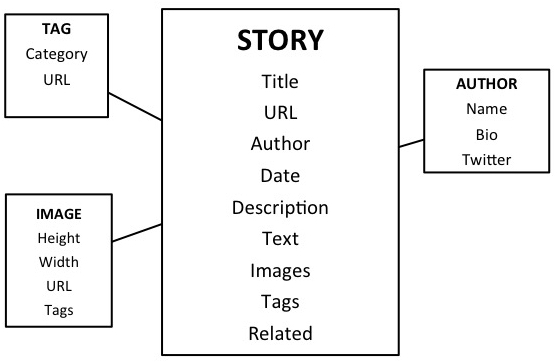
\includegraphics[width=300pt]{figures/storyschema}
\caption{Simplified metadata scheme for a typical news story.}
\label{fig:storyschema}
\end{figure}

% Also mention the IPTC Standard which is still in use TODAY.

The story has long been the basic unit of news, and so it tends to have a one-to-one relationship with the URL, the basic unit of the web. One section of the \emph{Innovation} report announces that the Times produces ``more than 300 URLs a day,'' using URL as a sort of ``thing'' word, their default unit of work.\autocite[27]{_innovation_2014} Most publishers will assign a ``canonical URL'' to a given story, which serves as its unique identifier, and often, practically speaking, it is the only information that a researcher or search engine can feasibly obtain about a particular document on the web.\footnote{While the researcher or bot crawler could, of course, request the webpage to get the information, each request can take several seconds and some processing power, so it becomes infeasible at a larger scale.}

But if stories contain multitudes, then why is the article the basic unit of information for news? An article can pull paragraphs from one source, photos and charts from another. It is an ecosystem of media itself, and it can contain other stories in turn. The news app Circa organizes its content around ``atoms'' of news: single facts, quotations, statistics, and images that can be reaggregated and remixed as needed. Systems like Circa's atoms or Vox's cards aim to create a baseline repository to build upon rather than recreate from scratch every time.

The sustainability and commercial viability of such approaches is still unclear, but the excitement around them speaks to a fundamental rethinking of how we organize news items and structure stories. A ``story'' can be a collection or dialogue of items; indeed, most stories already are. A journalist can still create, but also curate, collect, and contextualize, or allow users to do the same. All of these remixes and reuses can improve the classification and discoverability of the content in turn. Thinking of a story as a collection or mash-up offers a new framework of a story as a highly linked entity, one that can start to organize itself.

Adrian Holovaty, co-creator of the Django web framework and its now-retired ``benevolent dictator for life,'' sees a deep future in this new, structured approach to journalism. Holovaty wrote in 2006 that ``newspapers need to stop the story-centric worldview''; each story, he argues, contains a vast amount of structure that is being thrown away with every click of the ``publish'' button.\autocite{holovaty_fundamental_2006} He leads through several examples, such as: \begin{itemize}
\item An obituary is about a \emph{person}, involves \emph{dates} and \emph{funeral homes}.
\item A \emph{birth} has parents, a child (or children) and a date.
\item A \emph{college graduate} has a \emph{home state}, a \emph{home town}, a \emph{degree}, a \emph{major} and \emph{graduation year}.
\item A drink special has a \emph{day of the week} and is offered at a \emph{bar}.
\item A \emph{political advertisement} has a \emph{candidate}, a \emph{state}, a \emph{political party}, multiple \emph{issues}, \emph{characters}, \emph{cues}, \emph{music} and more.\end{itemize}

\noindent Holovaty links to context everywhere above, using hyperlinks to literally highlight the information that's otherwise locked away behind stories. Of course we don't need all of this context all the time, but we may really need \emph{some} of the context \emph{sometime}, and it's easier to structure it now than to unlock it later. The better structured this information, Holovaty argues, the more serendipity can foster new features and applications. Proper story scaffolding can lead to more happy accidents of ``wouldn't it be cool if\ldots'' later. Want to map the births and deaths of a famous family, or photos taken at a historic site, or the happy hours in a neighborhood? You might already have that information buried in your stories.

One example comes from the \emph{Boston Globe}'s March 2015 coverage of the Boston Marathon bombing trial. Data editor Laura Amico knows well that trials are far from linear stories; since they are told by lawyers, they unfold as a series of conflicting arguments. Trials present a proliferation of stories: the chronological narrative of the trial, the pieced-together narrative of the original event, and fragments of tangential narratives from witnesses and documents. Moreover, the Globe already knows about, and has written about, many of the key players in the bombing trial, through covering the bombing itself and its many witnesses, victims, and pieces of evidence. Amico and her team knew there was more than one way to tell this story, so they decided to focus on the facts: each witness, exhibit, and argument is entered into a spreadsheet, which can generate snippets of facts and entities---designed as cards---for later review.\autocite{mullin_how_2015} These cards can embed and contain other cards, or be combined to form a story. Such a framework is built for easy reuse; it recognizes the interlinked nature of events, and the stories that summarize and filter events. The coverage also highlights that ``structured journalism'' does not need to be adopted wholesale; it can work for one-off stories, events, and experiments as well.

Still, despite the news story's rigid structure and the limitations of indexing, the article is not disappearing anytime soon; it remains the core and canonical unit of online work. Link-based platforms and services like RSS and social media feeds still rely on conventional, stable, and consistent resources at given URLs. Still, some new forays into interactive, multimedia, and app-driven journalism enhance or bypass the URL and hyperlink---I will touch on these at greater length in the conclusion. My aim is not to suggest that we need to restructure the news story completely; only that we rethink how they work under the hood. Stories are not uniform resources, and they should not be uniformly tagged and categorized.

\subsection{From tags to links}

On the web, stories gain a new structure and unprecedented source of new insights through hyperlinking. Links---and their siblings, linked tags---allow for a new standard of citation, reference, and context provision for news. When used internally and indexed as first-order metadata on a story, a link can go beyond the footnote by linking in both directions, allowing readers to see who referenced the story; an old article in \emph{The New York Times}, for instance, can link out to more recent related Times articles, other publishers or blogs that picked up on the story, or conversations in the \emph{Times} forum or on Twitter. Linking offers great potential, not only for enlivening the reading experience, but for creating a traceable dialogue that can improve a story's discoverability in the future. A number of search algorithms, such as Google's PageRank and Jon Kleinberg's HITS system, create ``hyperlink-induced communities'' between websites, and the same principles can be adopted and expanded within news websites.\autocite[12. See also section 5.1.]{chakrabarti_mining_2003}

Organizing the web by link and tag has often proven more effective than trying to fit its contents into an overarching taxonomy or ontology. Google's PageRank algorithm was the lifeblood that made it the dominant search engine over rivals like AltaVista and Lycos.\autocite{shirky_ontology_2005} When Yahoo! began in 1994 as a hierarchical directory of useful websites, it seemed like a natural step. Computer users were accustomed to the tree-like document and file structure of computer systems, and the web replicated this in turn. Taxonomy allowed Yahoo! to build relationships between categories into its structure---parents, children, and siblings---which readily enabled features like ``related categories'' and ``more like this.'' But Google succeeded by crawling in the weeds rather than commanding from on high. For Google, the links sort everything out. Berners-Lee proved that networks could work with many links---and in fact, if you had a lot of links, as Clay Shirky puts it, ``you don't need the hierarchy anymore. There is no shelf. There is no file system. The links alone are enough.''\autocite{shirky_ontology_2005}

This is not a completely new phenomenon; long before Google's PageRank, scholars long relied on the footnote and bibliography to systematically track influence and dialogue, and networks of citations can be created through organizing and ranking by reference. This forms the basis for citation analysis, or bibliometry, a practice with a long history and strong conventions that I will dive into more closely in the following chapter. Its essential principle is that the more an item is cited, the more influential and credible it is. The online version is known as ``webometrics,'' and it applies certain new standards, weights, and details which online newspapers can take advantage of, both in measuring impact on the web and inside their own archives.

The tag emerges somewhere in between the category and the link, as a hybrid hierarchical/networked organizational structure. On one hand, tagging relies on an individual singularly classifying an object under a certain discourse. On the other hand, users are generally free to tag as many times as they want, and using whatever scheme they desire. Tags could range from ``World War II'' to ``articles I want to read.'' Studies and businesses alike have proven that at web scale, even with users tagging items for personal and idiosyncratic reasons, distinct and simple patterns emerge that allow for collaborative classification.\autocite{cattuto_semiotic_2007} These systems, sometimes called ``folksonomies,'' emerge as manifestations of the ``boundary infrastructures'' proposed by Bowker and Star.\autocite[See also section 2.1.]{bowker_sorting_2000}

Tags have their limitations; if another user tags an item ``World War 2,'' the system needs to recognize that it means the same thing as ``World War II,'' and publishers employ controlled vocabularies to avoid such ambiguities. Even controlled vocabularies don't always work: tags like ``George Bush'' are more challenging for a machine than ``Barack Obama.'' Some research has also shown that the first tags on an item are likely to influence future tags in turn, resulting in a sort of ontological groupthink.\autocite{cattuto_semiotic_2007} Still, whether a Flickr tag, a Delicious bookmark, or a Twitter hashtag, these crowdsourced approaches to tagging function as links between content; it is not about the tag itself, but the \emph{connection} being made to other content. This suggests that tagging is a crutch, a tacit recognition that all associations must be mediated through language. Taxonomists sometimes employ ``synonym rings'' to link related terms, but Shirky considers the possibility that syonymous terms aren't always desirable; perhaps the people who are searching for ``films'' would be better served by just seeing results tagged as ``films,'' and not ``movies'' or ``cinema.''\autocite{shirky_ontology_2005} This radical suggestion uses minor semantic differences as signals, but sometimes hierarchies are crucial; a user searching for movies set in Massachusetts would also want movies tagged ``Boston.''

The \emph{Times} sees tagging as core to its business, and the reason it has remained the ``paper of record'' for so long.\autocite[41]{_innovation_2014} This title was bestowed to them largely on the back of the legacy New York Times Index, which has offered an annual reference version of Times stories since 1913, still published in hard copy. There is no doubt that the \emph{Times'} tagging practices have helped them remain a library, information hub, and general authority on contextual information. But the \emph{Innovation} report sees them falling behind, adhering too much to the needs of the hard copy Index. They also note crucial limitations with identifying, splitting, and lumping categories; for instance, it took seven years for the \emph{Times} to start tagging stories ``September 11.'' Other times, topic relevancy changes; early stories about solar power might have been tagged ``science,'' but now the paper could have a dedicated ``environment'' or ``clean energy'' section or tag. Along with keeping up with topical drift, the \emph{Times'} team of librarians is required to shepherd about 300 new articles a day into the archive, making sure to keep them discoverable under any context. Tags can concern more than just the contents or event of a story---the Report suggests tagging stories by timeliness, story tone, and larger ``story threads''---but they admit that many of the more exciting tagging potentials would require them to ``better organize our archives.''\autocite[41-42]{_innovation_2014}

So the linking of the archive can occur not only through explicit hyperlinks, but implicit tags and entities that reside within the stories themselves. Most news articles rely on tagging to be connected to other media; if the \emph{Boston Globe} writes a story about New England Patriots coach Bill Belichick, an editor might tag the story ``football'' in order to place it in dialogue with other football stories, landing on the \emph{Globe}'s football topic page, and so on. But this belies a more nuanced dialogue between the words, images, and hyperlinks used within the story itself; a short story that has ``Bill Belichick'' and ``Cincinnati Bengals'' in the text is likely to be referencing a recent game or a trade, while a longer story that brings up his family members or his hometown is likely to be a biographical piece about his life and upbringing. Most stories are tagged manually, by an impatient reporter or editor on a tight deadline and according to a certain context. By combining modern natural language processing tools, a story can instead be automatically and dynamically tagged according to the myriad possible contexts that a user might search for, whether she is looking for stories about football, the Patriots, or Bill Belichick himself.

While tagging practices can be enhanced in a variety of ways, Stijn Debrouwere thinks that even ``tags don't cut it.''\autocite[``Tags don't cut it'']{debrouwere_information_2010} As an expert in news analytics and a co-creator of link-tracking platform NewsLynx, he knows well the limitations of the web and newsrooms' content management systems. His blog series ``Information architecture for news websites'' dives into the headaches that result when journalists think of stories as blobs of text in feeds and streams, rather than structured systems of facts and ideas that carry value in their own right. For Debrouwere ``each story could function as part of a web of knowledge around a certain topic, but it doesn't.'' Tags are our only window into content at the level of a story's metadata (which, too often, is all we have). For all their weblike strengths, they are still often inconsistent, outdated, and stale, and they give little indication of the meaning behind the relationship being formed. Debrouwere advocates for indexing these relationships: ``A tag on an article says `this article has something to do with this concept or thing.' But what exactly?'' Rather than tagging an article ``Rupert Murdoch,'' a tag has more value if it can say ``criticizes Rupert Murdoch.'' For Debrouwere, ``we don't need the arbitrary distinction between a label and the thing it labels on a website. Let's unlock the full potential of our relationships by making them relationships between things.''

Debrouwere also suggests using \emph{linked entities} instead of tags and labels. Natural language processing tools can find the entities---the people, places, organizations, events, and themes---in a given text with reasonable accuracy, and then link these entities in turn to knowledge bases like Wikipedia, IMDB, or any number of digital libraries, museums, and research institutions. This allows machines to infer the broader topic and detailed relationships from a given text. The result is a tagging system where a tag can double as a card or widget, linked in turn to other cards and widgets in a network of knowledge. This could be extended to events and phenomena as well as proper names and entities; some emerging systems can recognize phrases like ``Barack Obama announced his candidacy for president'' and ground it as as a unique, unambiguous newsworthy event, linked to other unambiguous entities (like Obama, and the POTUS) in turn.\autocite{nothman_grounding_2013} While this research has a long way to go, it is a promising start towards extending the notion of events as relationships between entities, and stories as relationships between their fragments.

Every story---whether a blog post, a map, a listicle, or an interview---has its own structures and patterns, each of which can be indexed and mined for future archival value. One of the most obvious and underexplored of such structures is the hyperlink. A year after publishing his ``Information architecture'' series, Debrouwere followed up by questioning many of his own allegiances; tags still don't cut it, but maybe linked tags and taxonomies don't either. He realized: ``The best content recommendations on news websites are inside of the body copy: inline links. With recommendations, you never know what you're getting. It's mystery meat. With links, a writer tells you why she's pointing at something the moment she's pointing at it.''\autocite{debrouwere_taxonomies_2011} It is better, Debrouwere imagines, to draw on the connections from these links than to rely on automated recommendation engines to organize content. Journalists are better at explaining and contextualizing than they are at tagging and structuring, which are a librarian's craft. Debrouwere knows that newsroom developers are building for journalists, and he ends by asserting that he wants to build ``prosthetics, not machines.''

Another under-mined source of insight lies in the plethora of ``human-generated lists'' (as Google calls them in one patent) around the web.\autocite{franks_discovering_2012} Whether collecting articles, photos, books, songs, or tweets, people obsessively collect and curate, and some are known experts at doing so. These range from Amazon wish lists to mixed-media stories on Storify. Thinking of lists as links between contents, weighted by expertise, leads to interesting potentials. The title of the list, or its other metadata, could tell us more about the context behind the link; a list of local Mexican restaurants is linked by type and location, while a list of my favorite hip-hop albums of 2014 is linked by year, quality, and musical genre. The \emph{Times'} \emph{Innovation} report suggests allowing users to create lists, since it could allow for deep interactivity without risk to their brand; such a system could leverage readers' collective wisdom by asking users to specify the context behind their lists as well.

A human editor who is tagging a story is equivalent to the archivist in the library, attempting to predict every possible way that a user might search for the story in the future, whether it's ``Sports'' or ``Breaking'' or ``Opinion''---and editors don't have the extensive training and professional expertise that comes with being a librarian or archivist. Journalists are trained to explain, contextualize, and curate rather than structure and tag. Given the impossibility of explicitly and expertly tagging in advance for every possible present and future use, as well as the arbitrariness of tagging \emph{the story} instead of its constituent parts, we can turn to entities and links as supplements to categories and tags in the newsroom archive. These play to a journalist's strengths, and augment rather than replace the human touch that comes with inline links and curated collections.

These web-native and polyhierarchical approaches to classification reflect the growing need for newsrooms to find weblike ways to organize their stories. Shirky is a champion of the tag, but he recognizes that organizing by taxonomy and ontology is sometimes preferable; namely, with a small corpus and expert catalogers.\autocite{shirky_ontology_2005} This could have described a pre-web newsroom, but no longer: the publisher's corpus has expanded and linked beyond measure, and its ranks of expert catalogers are rapidly dwindling. Meanwhile, readers expect an increasingly rich, contextualized, and personalized approach to information. This suggests a need to adopt new schemes, ones that leverage automatic and dynamic tagging, linked entites, image recognition, and the knowledge of experts and crowds.

\section{Conclusion}

The linked archive, when considered on a massive scale, is a quixotic endeavor along the lines of the Radiated Library or Project Xanadu. We can't predict all possible links between every possible piece of content. Likewise, no automated system is perfect, and a computer cannot fully follow many of the nuances and changes that languages and topics undergo. Linking the archive demands a symbiosis of content, business, and technology; it requires considering journalist-as-archivist and technology-as-prosthesis. Linking the archive requires making more structured and explicit, and subsequently mining the web of references that already reside in the stories; it requires a rethinking of the practices of journalists and editors, as well as an adoption of new tools and techniques.

The linked archive borrows from, but is distinct from the notion of ``link journalism'' or ``networked journalism.'' As a term popularized by Jeff Jarvis to refer to the growing citizen journalism movement, link journalism has also led to Jarvis's succinct motto of ``Cover what you do best, link to the rest.''\autocites{jarvis_new_2007}{jarvis_networked_2006} Building on this idea, Charlie Beckett posits that linking between sources leads to editorial diversity, connectivity and interactivity, and relevance.\autocite{beckett_editorial_2010} A linked archive turns the conversation inward---as Mark Deuze and others note, inlinks are vastly different from those that point out---but they can adhere to the same principles of diversity, connectivity, and relevance. While inlinking may seem nepotistic and selfish, this is not the case if the archive itself links out in turn.  A user doesn't always know exactly what he or she wants, and a linked archive can work with a user to surface it. If the archive doesn't have the resource a user needs, could it at least point the user in the right direction? Could it interface with other knowledge bases to retrieve the answer?

It is unhelpful to have a massive, borderless archive, but linked archives can expand their borders strategically through clever use of APIs. Publishing websites rarely operate alone; they rely on a plethora of third-party platforms and services for analytics, sharing, commenting, and recommendations. One could similarly integrate with APIs that offer archival resources from around the web, such as results from Google, Wikipedia, Flickr, or resources from digital libraries like Europaeana and the Digital Public Library of America---not to mention partnering with other publishers to merge archives or indices. If a user is searching a publisher's website instead of Google's, it is likely because she wants more context than a mere list or index of items. A user should be able to see response articles, comments, tweets, timelines, images and videos, from around the web (as long as these are visually separate from the main content to avoid confusion). Otherwise, users will continue to go to Google and Wikipedia for information. The linked archive is therefore intricately indexed on a small scale, but also effectively connected on a large scale, seamlessly interfacing with other archives and collections around the web.

%In the following chapter, I will consider the publisher's main window into the archive, and possible new standard for classification: the hyperlink

% \section{Context in context}

% Structuring and linking the news cannot happen through technology alone. One reason that newspapers lacked a citation convention before the web is because journalistic practice didn't require it; while scholars read and cite articles, journalists traditionally go into the field and gather quotes. These are not so easily cited; a well-organized journalist could keep recordings of sources and, for instance, link to a snippet of audio when adding a quote, but this isn't always possible. Journalists may also be reticent to link because they feel they don't need to; sometimes journalists need sources to remain anonymous, obfuscated, or off the record. Most journalists agree that linking manifests many core tenets of journalism, but forcing a journalist to obsessively link to every source would stifle journalistic practice.

% Still, journalists are increasingly citing sources that are already published, whether documents on DocumentCloud, data points from an open government database, or aggregated information from other news articles. New journalistic practices thus lend themselves well to structuring and linking to sources to position a story; the challenge is, in part, in shifting journalistic focus. A journalist might be more apt to say that a court hearing occurred ``last week,'' but it is more archivally valuable to say it happened on ``December 12, 2014.'' This doesn't necessarily require changing the prose in the story itself, but a semi-automated process could occur when publishing a story that suggests these structures behind the scenes.

% Named Entity Recognition and topic modeling tools can't do all of the work for us; there are too many missed signals and false hits. But a quick widget or plugin that works \emph{with} a reporter or editor to structure a story could prove fruitful. The challenge remains to convince editors of the value of this, and spend the extra minute verifying a story's structure.

% Much of the debate surrounding archives and explainers strikes at the heart of the role of journalism, both on the web and as an industry and institution. Michael Schudson frames the rise of popular newspapers in the 1890s as a pull between two journalisms, one telling ``stories'' and the other providing ``information.''\autocite{schudson} Which of these functions is the primary goal for a news outlet? This question remains critical today, with most news operating on a sort of continuum between these points. Information focuses on the facts, while stories serve an ``aesthetic'' function. But in general, a faster-paced breaking event (such as occurring over an AP wire or a Twitter feed) will result in information, while contextualized longer-form histories and interactive multimedia (like a \emph{New York Times} interactive or \emph{New Yorker} longread) skew towards stories.

% Interactive digital multimedia emerges somewhere between these scales, providing information that allows users themselves to create stories. Interactives carry the promise of deep contextual information along with narrative elements, but given the extremely time-consuming process of building an interactive piece, they tend to accompany events planned far in advance and guaranteed to drive traffic; you're more likely to see an Oscar's, World Cup, or presidential primary interactive feature than rich multimedia surrounding breaking news such as a plane crash or terrorist attack. While both breaking news and deep interactives seemingly exist to provide information, the interactives offer a  proliferation of stories to go with it.

% Such interactive elements are rich with the potential for re-use. Some of the pieces stay relatively ``evergreen'' in both content and structure, proving useful months or years later. They also incorporate collections of media that, taken together, form a network or ecosystem of resources that allow for a new view into digital archives, focused on what media you're utilizing and citing as much as what words are on the page, or what desk you're reporting from. As such, deeply linked multimedia stories can better structure an archive; but can the depth and immersion found in explainer sites scale to work with breaking news and ongoing scoops as well?

% \subsection{Paywalls}

% While many traditional media publications are recognizing the potential role of archives in their shift to digital, they have tended to silo away their archival resources behind paywalls. This is the most literal interpretation of gaining value from one's archive, and it is an understandable choice given the few avenues for them to make money on the web. But paywalls are just one of many possible ways to extract value from archives, and there's more than one way to make a paywall.

% One problem with the way that publishers deal with their paywall now is that they have few ways of measuring ``successful'' archive diving. Like many publishers, Time.com requires a paid subscription in order to access their online Vault. But say a registered user is clicking through the Time Vault. Did she sign up for the subscription just to see the old issues? Is she there on a dedicated research project, or is she just browsing?

% Archive paywalls tend to be very limiting; while publishers will occasionally lift the paywall on relevant archival stories, it is usually impossible to even preview an archived story. This prevents interested users from even testing out the interface or getting curious in the archive in the first place. As online publishers experiment with paywall methods, they should keep in mind their older stories.

% Some archives are more open than others. The New Yorker opened its archives for the summer of 2014, free of charge, as they built the paywall system. The archive is now back behind walls, but the summer experiment seemed interesting. How much were users diving into the archives? How were they browsing the archives--through search or serendipity? Did opening the archives encourage people to think and write more about the New Yorker's rich history?

% % Can I talk to the new yorker abt their experience and write about it here?

% A publisher's archive will often turn up in specific articles geared towards history. At Time.com's Vault, editor/curator Lily Rothman digs out stories and quotes from the history of Time, ranging from historical interests (``Read TIME's Original Review of \emph{The Catcher in the Rye}'') to ephemeral oddities (``13 Weirdly Morbid Vintage News Stories''). Time assistant managing editor Samuel Jacobs likened Rothman to a radio D.J., highlighting singles from the archive to entice readers to pay for the whole collection.\autocite{}

% Other historic deep dives might occur in weekly columns or ``long history'' forays by individual journalists. A Sunday Times article, for instance, might take a historic look at a particular person, neighborhood, or community. These projects have a chance to draw attention to the past through curation as well, by drawing out and resurfacing old stories, photographs and statistics. These projects are a promising start, but they tend to be isolated endeavors, relegated to a single story. Sometimes willfully nostalgic, they do not bring the archive fully into dialogue with ongoing events, whether in the research or design process. Topic pages suffer from lack of organization and explanation.

% % Find a few examples here. Local interest stories etc. e.g. history of Whitey Bulgur, Boston's bids for the Olympics, or neighborhood deep-dives.

% 

% More generally, news' perpetual focus on the \emph{new} and \emph{now} keeps news publishers in the mindset of serving as information providers rather than knowledge repositories. This results in news delivered in story format, through wires, feeds, and streams. These are one-dimensional channels and metaphors, delivering information in a straight line and single direction. But information is more understandable, sustainable and useful if it's in more than one dimension, structured as a tree, rhizome, or web. Internal news archives have the potential to provide richer, faster resources and connections than the web as a whole, or its indexers (like Google or LexisNexis). This can drive traffic back to the site in turn, and bolster the publisher's authority as an information source. Legacy news publishers are rightly proud of their long histories of stories, photos, and notes; they could do well to show it off rather than hide it away behind paywalls. For publishers, opening access to their past could contribute to solidifying their status in the future.

% \subsection{The Scoop Effect} % Dear lord find a better term for this

% The time is ripe for news and history -- content and context, feeds and archive -- to collide. News outlets have long obsessed over the ``scoop'', being the first to break a story, and indeed these breaking stories still drive a great deal of traffic. But publishers are increasingly scooped in turn; stories break immediately on social media, rather than the next morning in the newspaper. % Can I coin a neologism for this? The "break effect" or something? So that I can keep referring to it in the next couple pages without driving myself crazy
% Emily Bell argues that social media and ``these super platforms ARE the free press, taking over many of the functions of the mainstream media. Social networks are now attracting the same pressures and challenges at a much larger scale that journalism and civic media has wrestled with for years.''
% This is having a profound effect, of course, on publishers; where does the media fit in here? But it is especially affecting the research process, skills and news lifecycle for both journalists and editors/strategists.

% For journalists, it has increasingly destroyed the stereotypical image of the reporter with a notepad in city hall. The increasingly real-time nature of scooping has led to reporters scouring Twitter as much as being in the field; even communication with sources increasingly occurs via email or tweet. The increasing presence of ``explainer'' and ``data journalism'' likewise speaks to this need; reporters must to wade through massive amounts of information in fast, efficient ways in order to uncover possible news stories, which requires very strong digital research skills. These are skills that librarians have been practicing for centuries, and a well-organized and linked archive can help reporters immensely with this research process. The data journalists thus emerges as an amalgam of reporter and librarian.

% For editors and newsroom strategists, it has shifted the role of the journalist and the news publisher to explainer, data-gatherer, and context-provider. Picture a newsworthy event occurring as the epicenter, and the reporting that occurs around it as a set of concentric circles around the event. Towards the center, one might find tweets, wire reports, and quick announcements. At the edge, there are longform pieces, explainers, multimedia work and data-oriented stories that help draw immediate events into larger phenomena. While the scoop remains crucial and breaking news draws traffic, news outlets can no longer serve as raw information providers, with no context. For a publisher to stand out, it is crucial to bring ongoing stories into a larger dialogue and conversation.

% % Coddington 2014 WikiLeaks article. Also articles from Ethan's class. "Sense-making" rather than "information-gathering"
% % Also Boczkowski 2010 talks about recycling content ("News at Work" book)

% \subsection{Explainers}

% This focus is not limited to legacy media, as the rise of ``explainer journalism'' and context-based reporting emerges as the other side of this coin. \emph{The Nation}'s editor and publisher Katrina vanden Heuvel suggests that ``a clever use of archives is kind of an explainer 2.0.''\autocite{} The goal is to provide knowledge, not news.

% The concept of explaining the news is not new. A 2001 Pew Center survey of newspaper editors concluded that they wanted to be ``news explainers'' first and foremost, ahead of ``news breakers'' or ``investigative watchdogs.'' But in a 2008 article called ``National Explainer,'' Jay Rosen accused editors of not staying true to their mission: journalists are not good at explaining the news and providing context. Instead, they focus too much on incremental and episodic updates, many of which go over the head of readers who haven't been following. Rosen likens the process to pushing software updates to a computer that doesn't have the software installed.

% Rosen argues that while journalists are paid to report the news and not explain it, they should also be giving background and context to larger stories. Journalists ``don’t do a very good job of talking about the beginning and what got us to this point where it became news,'' according to Alex Blumburg of \emph{This American Life}. Even the occasional explainer that gets it right ends up in the flow of the same old information; Rosen argues that explainers like David Leonhardt's credit crisis piece in the New York Times ``should have been a tool in the sidebar of every news story the Times did about the mortgage mess.'' The little ``what's this?'' link is ``not about web design. That's a whole new category in journalism that I fear we do not understand at all.''

% Rosen also points out that such explainers are helpful for other reporters as well as the public, influencing news and information flow across the pipeline. A Times explainer, for instance, can reach a reporter who is informed by it as he or she interviews local officials. Calling it a ``scaffold of understanding,'' Rosen suggests that we ``start with clueless journalists'' in the path towards providing context, and went on to create explainthis.org, for people to admit what they don't know to journalists who are ``standing by.''\autocite{rosen_2008}

% Explainthis.org, now defunct, was like a library reference desk, staffed by the public and monitored by journalists. A peer of StackOverflow and ancestor to Quora, it is organized around questions rather than topics, discussed by the public and monitored by journalists. It requires someone to be curious enough to ask the question, however. Rosen touts the ability of explainers to generate interest in a topic, but here we're already expected to be interested.

% At a South by Southwest panel in 2010 called ``Future of Context,'' Rosen outlined the reasons explanation is needed and why it wasn't taking off. He cited both design and institutional problems; the prestige and real-time excitement of breaking (rather than explaining) news, as well as the explainer format getting lost in the shuffle of other news items.\autocite{rosen_2010} Metrics like clicking, watching, and even spending time on a site are not measuring the level of understanding or knowledge gained.

% The panel opened with NPR's Matt Thompson, owner of former contextual news blog newsless.org, arguing that we need more ``systemic information, not episodic info.'' Systemic information could include lists, charts, and maps that stay valuable well after the episodic news is irrelevant. Tristan Harris of Apture says, ``my background is computer science. You never do work that you can't re-use.'' He suggested an ``object-oriented'' approach to journalism with an eye towards sustainable, continuously updating tools and widgets that keep a reader informed. News is organized around stories rather than objects, resulting in streams rather than systems. A systemic, object-oriented approach to news places the context in the center.

% The panel concluded with Harris suggesting a wiki-like approach to journalism, which a big news organization like the New York Times would have the power to sustain. When Kramer asked ``how is this more than links?'' Thompson replied ``Links can be part of it.'' So can wikis, embeds, collections, and related articles.


% ``The context should be the foundation. The systemic stuff should be what you can access first. The episodic stuff is what should be the more info. We “ghettoize” topics pages on our sites, by creating a topics section. When the public just finds just a random collection of links on a so-called topics page, “the quest for context everywhere is set back,” Thompson argues. What would a site look like if it were structured around systems instead of stories?

% Journalists may think, we’re doing so much and now you want to provide context!? Think like an engineer. Make it an imperative to do work you can re-use to provide context. You can use that subduction plates info graphic again and again with every story you write about earthquakes. It’s redefining the notion of “today” value. You’re writing something TODAY that’s only appending something that’s already valuable. Engineers don’t do work they can’t re-use. Do work you can use next time.''

% Chuck Peters, CEO of the Cedar Rapids Gazette:

% ``I can’t see providing that context without changing how we create information in the first instance. Any factual element (photo, incident, quote, data, etc.) can be relevant to numerous contextual narratives. So each of those elements needs to both “stand on its own” and be tagged with as many potential relationships as possible\ldots We usually create information today in locked-down packaged articles, which block the easy flow of the elements between and among narratives.''

% Finally, in an article entitled ``Swimming lessons for journalists,'' PBS's Amy Gahran asserts, ``today’s journalists can---and probably should---consciously shift away from jobs that revolve around content creation (producing packaged `stories') and toward providing layers of journalistic insight and context on top of content created by others (including public information).''

% % Criticize explainers a bit. ``Everything you need to know about x'' sounds final; it runs counter to the very idea that knowledge is infinite, interlinked, and flexible/elastic/malleable. It might not be everything you need to know tomorrow. It might be more or less than you need to know depending on what you need. http://pando.com/2015/01/20/how-rap-genius-and-explainer-sites-are-killing-music-journalism/
% % It turns out that smart, easy-to-digest journalism doesn’t lend itself so easily to the fast production cycles of Internet media, which requires writers with little specialization to quickly educate themselves on a topic using Wikipedia or other secondary sources before regurgitating it back to the public. % "It keeps the reader at arm's length as an outsider looking in"

% % Problem with constantly-updating news: it might make it feel less consequential to publish something erroneous. How do you trust something without an official publish date?
% % Explaining is different from aggregating; and it can seem final and complete, the opposite of what's intended here

% \subsection{Vox}

% At the start of 2014, Ezra Klein left his position at the head of Washington Post's Wonkblog to start Vox, a news site that aimed to make context a first-class citizen of web journalism. Vox's mission: ``to create a site that's as good at explaining the world as it is at reporting on it.''\autocite{} Vox hopes to take a step back from the immediate news event and place it in a larger phenomenon. Taking the long view on stories also gives them an eye towards sustainability; Vox's topics are built around what they call ``card stacks.''\footnote{See http://www.vox.com/cardstacks.} Cards have titles like ``Everything you need to know about marijuana legalization,'' or ``9 facts about the Eurozone crisis,'' and each card is divided into question-driven subsections like ``What is marijuana decriminalization?'' Readers can navigate sequentially, or dive from question to question, going through Vox's explanations and photos. The final option is always the same: the ``Explore'' button takes the reader back to the top of the stacks.

% Vox's card stacks house a growing and morphing repository of knowledge. They are a public archive, like a Wiki but with more authorship intact. At the end of each card, Vox offers a link to email the author/curator of the card stack. For Vox reporters, starting a stack is also a pledge to maintain it. Vox also give a summary of changes made to the card (full versioning, they say, is coming soon).

% The goal is not to replicate Wikipedia, but more like a wiki ``written by one person with a little attitude,'' as Vox co-founder Melissa Bell put it. It's obeying the rules of journalism rather than ``no original research.''  Klein has Wikipedia in his sights, suggesting in the New Yorker that ``I think it's weird that the news cedes so much ground to Wikipedia. That isn't true in other informational sectors.'' By combining incremental news with an evolving repository, Klein hopes to gain the best of both worlds: ``the card stacks add value to the news coverage. And the news coverage creates curiosity that leads people to the card stacks.'' This follows Rosen's idea that explaining the news can generate future interest in incremental updates. For Klein, ``the biggest source of waste is everything the journalist has written before today.''\autocite{nyt_vox_melding} 

% For Klein, there is a distinct need, like Rosen saw, for a website that takes a step back and explains the news. In his words, ``The more folks in the media feel like it's beneath them to answer questions like ``What is marijuana?'' or ``What is Ukraine?'' the more we don't have to compete with them.''

% Vox has accompanied other ``explainer'' and data-focused websites, like Nate Silver's FiveThirtyEight, and The New York Times' The Upshot. Soon after Vox's launch, Craig Silverman wrote ``Why Vox (and other news orgs) could use a librarian,'' suggesting that Vox had ``a huge challenge, due to the rapid decay of facts.''.\autocite{}  Some of these facts may not even be obviously newsworthy, such as if an academic research paper changes a fact in an explainer on Alzheimer's care. Who is going to keep everything up to date? ``Someone at Vox is going to need to know which card stacks to update when,'' and how to keep the explainers updated with minimal maintenance.

% % Evergreen experiment at Vox http://www.vox.com/2015/1/15/7546877/evergreen-experiment

% % How to tie data journalism in with explainer journalism? With multimedia/interactives?

% % The ``tabloidization'' of news a la Emily Bell: "The demands of web scale economics have torpedoed the local news model". Can explainers and deep archive dives help bring local interest back to news reporting? How can news services provide local info too?

% % Herbert Simon "attention economy" in 1971 -- tied to Xeroxing. His concerns then are not new (information overload, attention economy)...but has the web's default state of copying exacerbated his concerns?

% \subsection{News Libraries}

% At a 2001 summit on news libraries, futurist Arthur Harkins suggested that in order to stay relevant, news librarians should ``leave the information management functions to automation'' and instead focus on ``the ability to put knowledge into context and to synthesize information.'' The librarians focused on solutions like structuring incoming stories, helping merge mixed media operations and create new revenue opportunities from older assets. teaching journalists the necessary research and technical skills. Finally, the librarian's task is largely to tag; to structure stories for future discoverability and reuse, by both journalists and the public. Some news libraries, like the Boston Globe, used to manually tag their stories, but no longer do.

% Today, many of these skills are expected of new journalists at the outset. Such reporters arrive armed with years of internet research skills, though some of it with Google over specialized databases. Leslie Norman, former librarian at the Wall Street Journal, suggested, ``I see the news library as it once existed as probably dying, but in many newspapers, it's evolved into something else.''

% Although news libraries are a dying breed, some libraries and cultural heritage organizations are making promising digital inroads into news. Old newspapers provide a rich archive of both historic resources and incidental ephemera like sports scores, weather reports, advertisements and small human interest stories. This gives historians a glimpse of a day, with the major phenomena of the day mixed in with everyday events.

% Most of these projects are aimed towards the serious researcher, but they also point towards ways to engage casual browsers and fans of history. The National Library of Australia's Trove collection features 370 million resources; primarily, Australian newspapers ranging from 1803 to 1954.\footnote{http://help.nla.gov.au/trove/building-with-trove/api} Their API allows programmatic access, which in turn leads to the TroveNewsBot, an irreverent Twitter bot that can search the collection and yield a personalized result. Similarly, the Digital Public Library of America's DPLA Bot and British Library's Mechanical Curator both post random resources from their collection, aiming to inject a serendipitous sense of the past into the present.

% Newspapers would do well to merge increasingly with digital cultural heritage institutions and library APIs. 

% or they argue that ``the software newsrooms have adopted in the digital age has too often reinforced a workflow built around the old medium.''

% \subsection{Promising starts}

% Some initiatives and organizations are taking promising steps towards linking their archives. The New York Times R\&D lab recently released a tool called Madison that aims to crowdsource insight about the ads in old Times issues. Starting with the 1950s, the tool asks users questions about the ads that they see, with the aim of adding structured metadata to otherwise difficult-to-parse texts. The team even released the underlying crowdsource platform as an open-source project, allowing others to run their own crowdsourcing endeavors. This is a promising opportunity for publishers who have the scale and user base required for a crowdsourcing project.m

% % Could I ask the Times how that's going? If they have similar projects?
% % Add some data about how it's progressing anyway

% % Vox Chorus
% Vox's Chorus platform is another promising endeavor in structuring archives. Beyond the sustainable mind to data that is Vox's card stacks, Chorus helps reporters better structure their stories, from adding smart tags to media and widgets.

% % Can I find out more about Chorus? Can I even see how it works?...

% % Photos
% Some promising endeavors are coming from small starts. Take a collection of already-related stories and build nuanced links between them. Or hone in on a single aspect of a linked collection -- for instance, geographic data -- and aim to structure that first. Projects like MapCake -- which automatically creates maps out of structured location tags -- show how effective it can be to focus efforts on structuring one media type. Sites like National Geographic are likewise well primed for beautiful photo archives, which can be watermarked and travel with articles and social media posts. It makes sense for such sites to focus on structuring their photo archives first and foremost. Radio and podcast-oriented sites could do well to take advantage of services like PopUp Archive

% Finally, there are many digital libraries beginning to offer resources and services; quotes, images, and videos. These have the potential to expand the borders of a news archive. The Digital Public Library of America, JSTOR, Flickr, PopUp Archive; all of these sites have useful resources for both reporters and readers. Many also have APIs that would allow easy integration with existing content discovery systems.


% Trends happen in cycles, and the news follows; the news is often repeating itself. Even something seemingly new like data journalism is a holdover of ``precision journalism,'' something that few news stories explaining the trend will point a reader to. Sometimes old documents, whether leaked or declassified, can refuel an old story and paint it in a new light. Other times, new cultural events will conjure up the old; when \emph{12 Years a Slave} was released, the New York Times unearthed a story about its namesake, which then went viral on Gawker.
